\label{sec:nueselection:inclusive}

The aim of the inclusive charged-current electron neutrino selection is to select electron neutrinos independently of their final state and energy. The selection performance is approximately 20\%, leading to 250-300 electron neutrino's in the Run 1-4 data-set. The purity without CRT is $\pprox$

\subsubsection{Pre-selection}

\begin{figure}
    \centering
    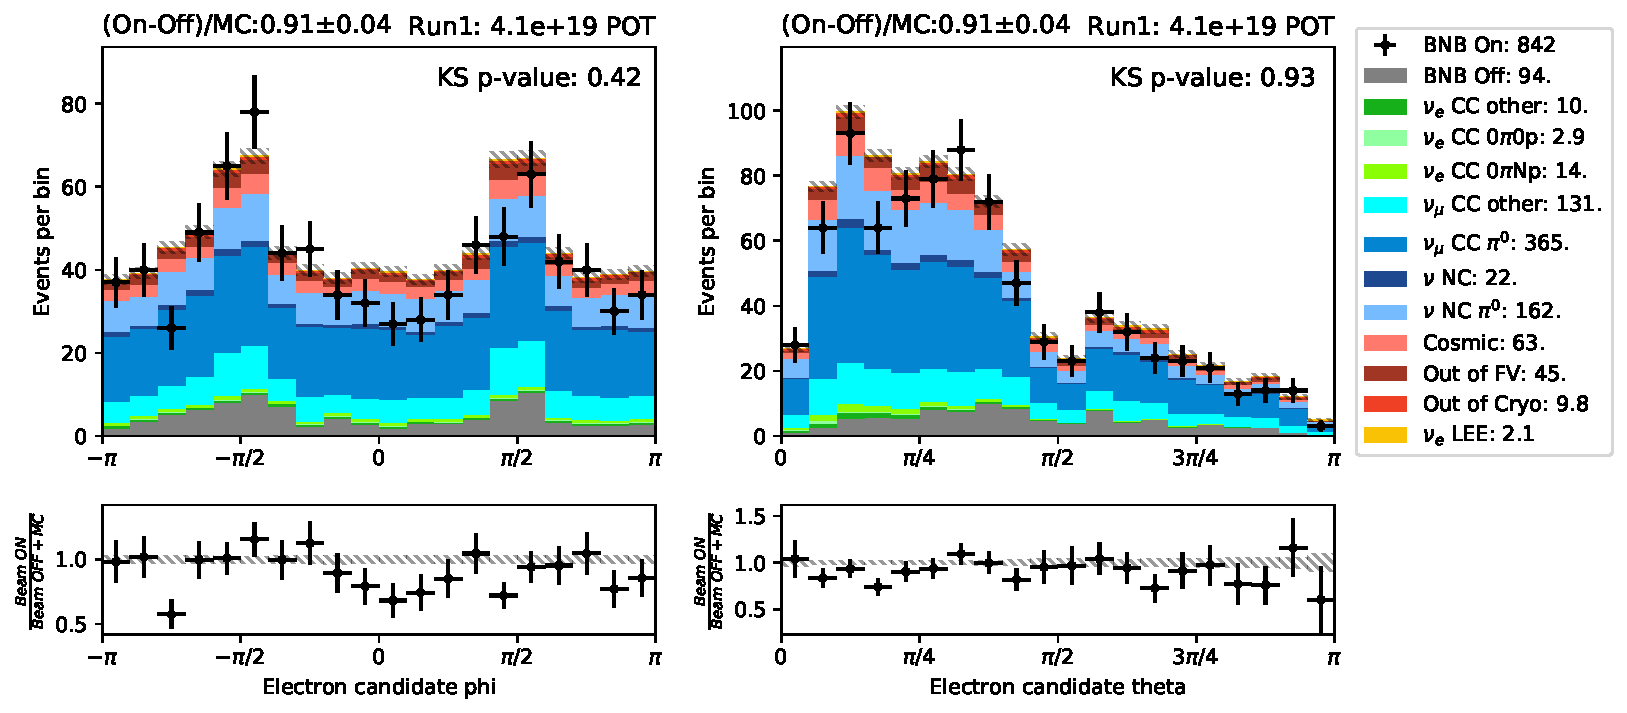
\includegraphics[width=\textwidth]{NueCCsel/Images/run1/pre_angles.pdf}
    \caption{Caption}
    \label{fig:pre_shower_E_pdg}
\end{figure}

\begin{figure}
    \centering
    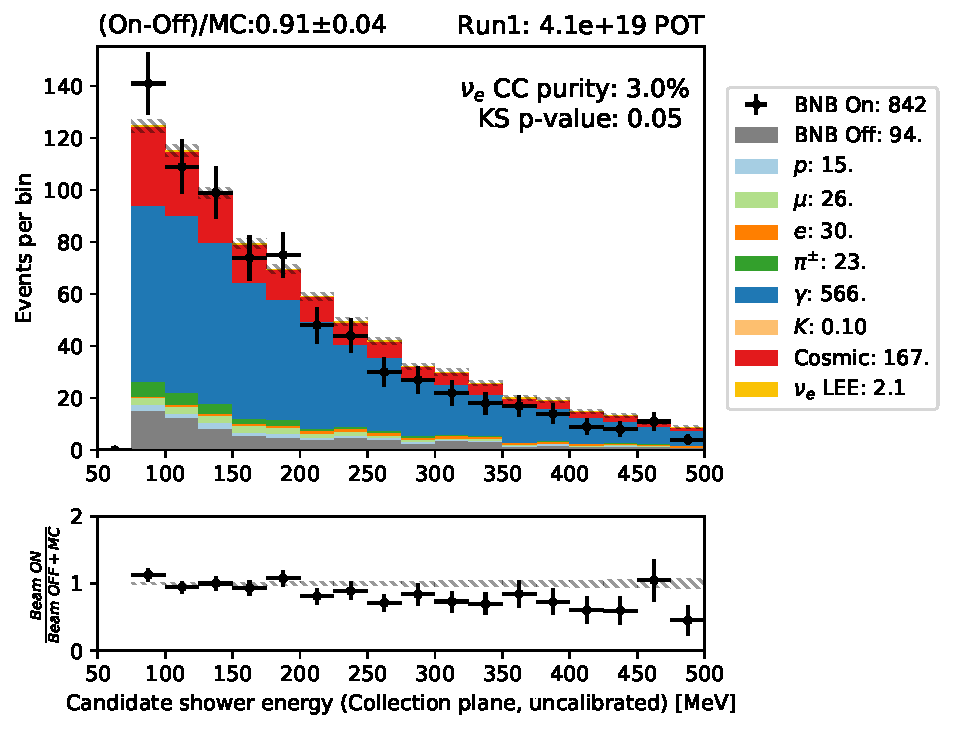
\includegraphics[width=0.5\textwidth]{NueCCsel/Images/run1/pre_shower_E_pdg.pdf}
    \caption{Caption}
    \label{fig:pre_shower_E_pdg}
\end{figure}

\begin{figure}
    \centering
    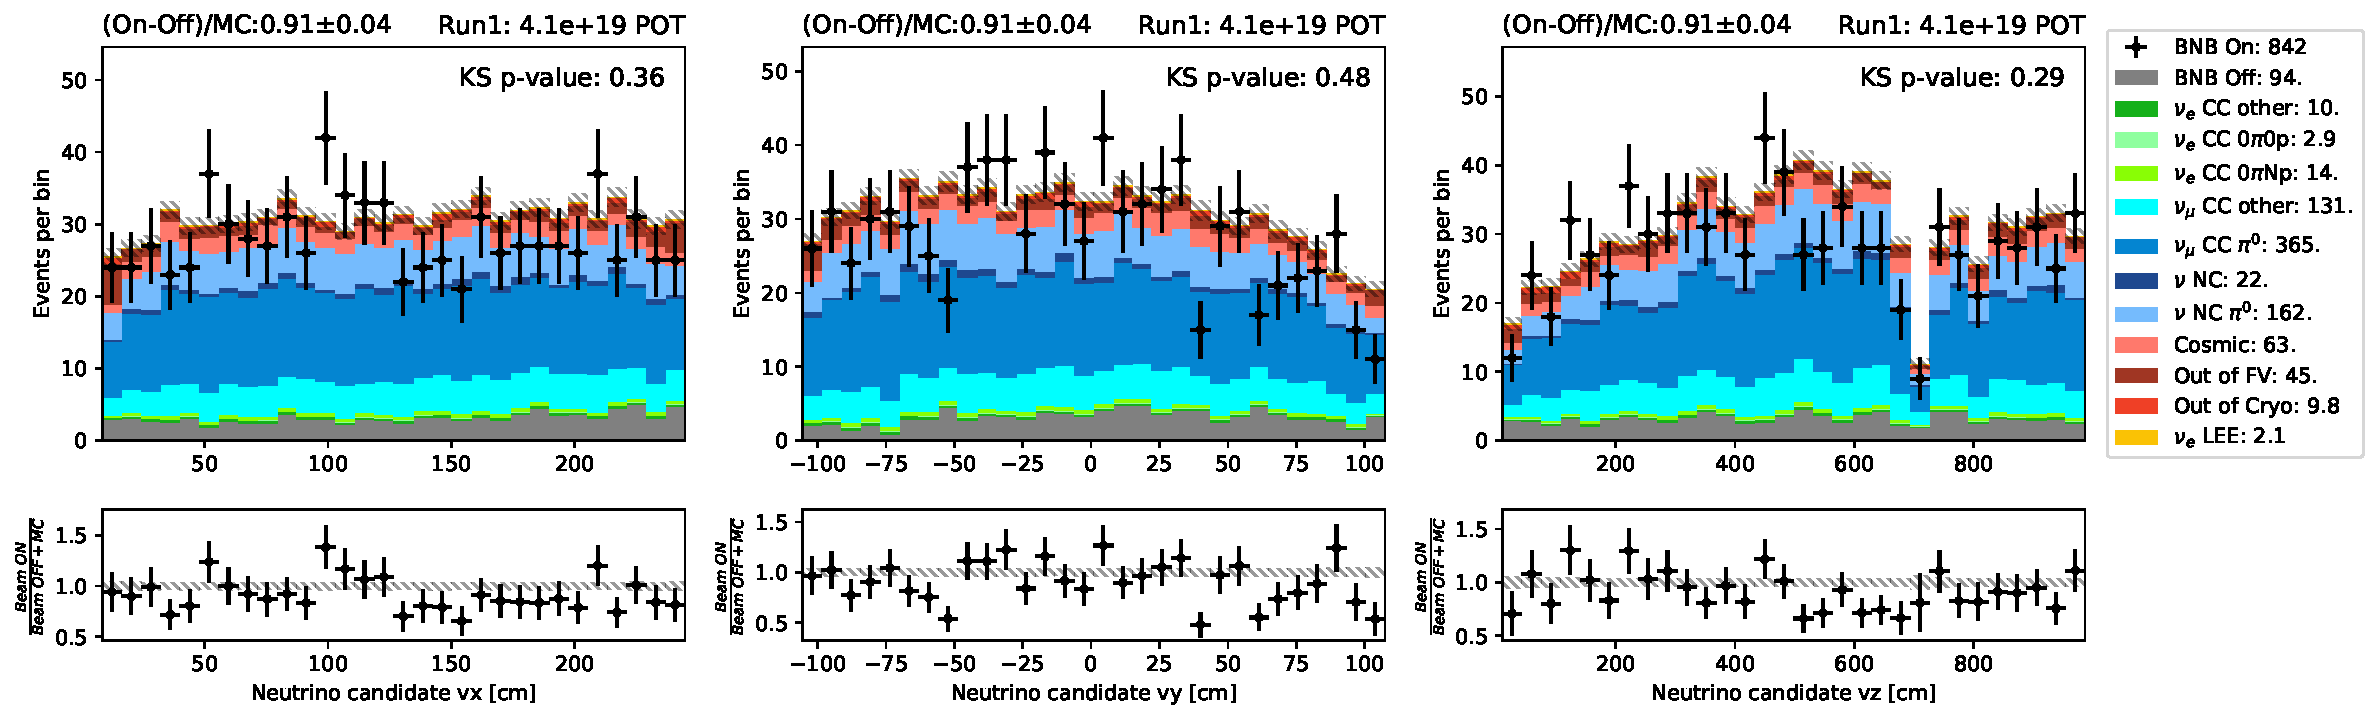
\includegraphics[width=\textwidth]{NueCCsel/Images/run1/pre_vtx.pdf}
    \caption{Caption}
    \label{fig:pre_vtx}
\end{figure}


\subsubsection{Electron Candidate Tagging}

\begin{figure}
    \centering
    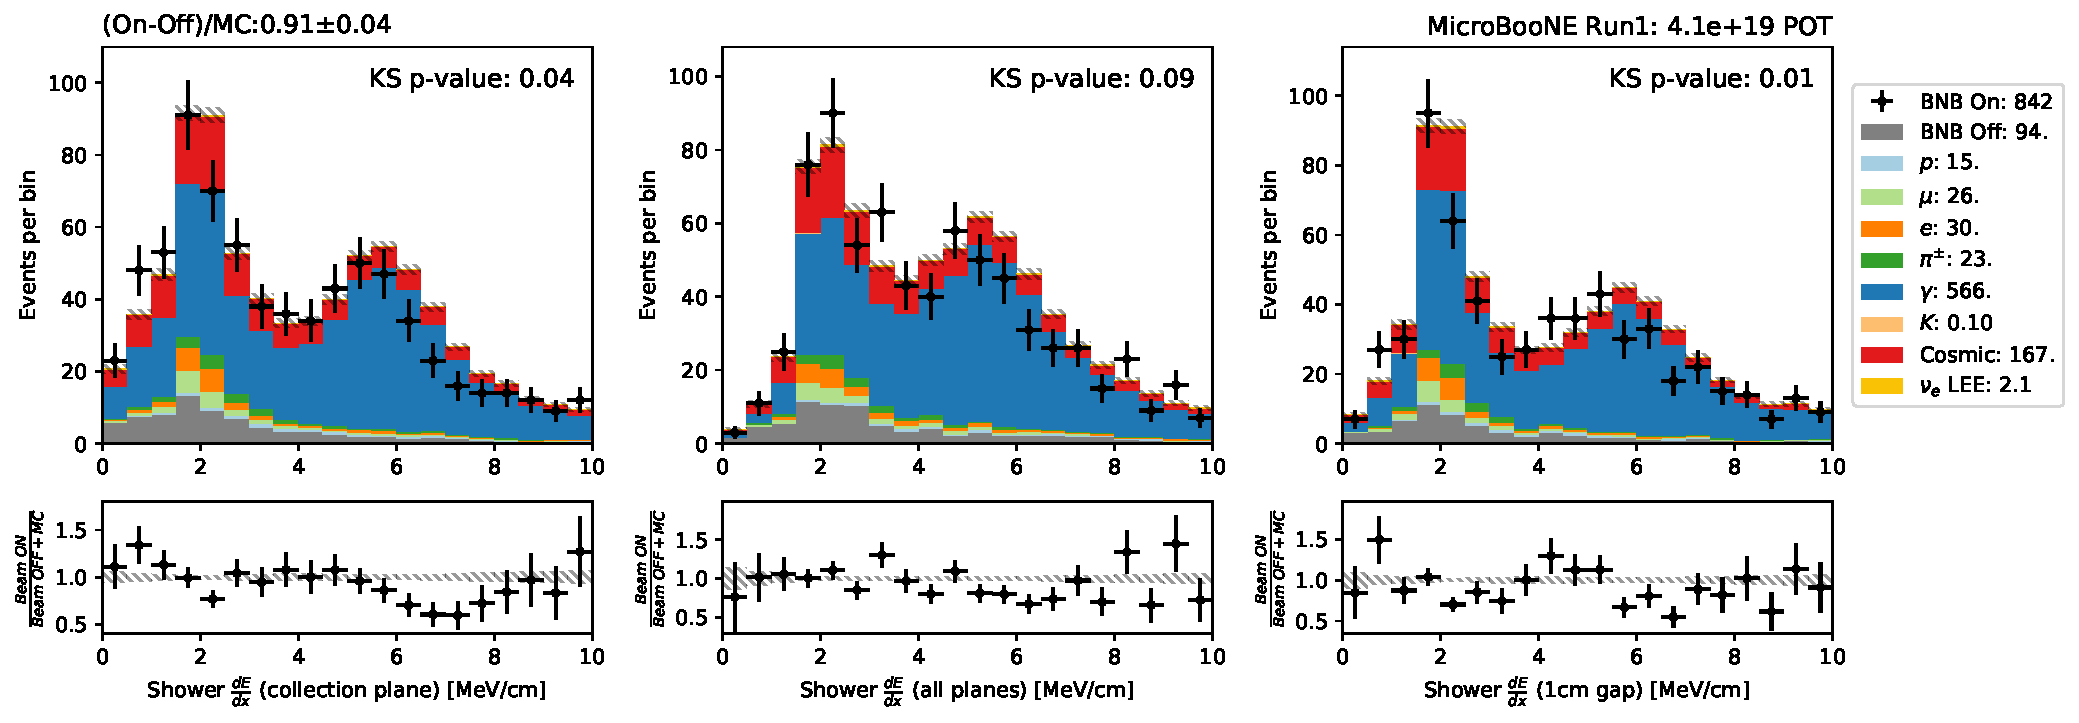
\includegraphics[width=\textwidth]{NueCCsel/Images/run1/e_cand_dedx.pdf}
    \caption{Caption}
    \label{fig:e_cand_dedx}
\end{figure}

\begin{figure}
    \centering
    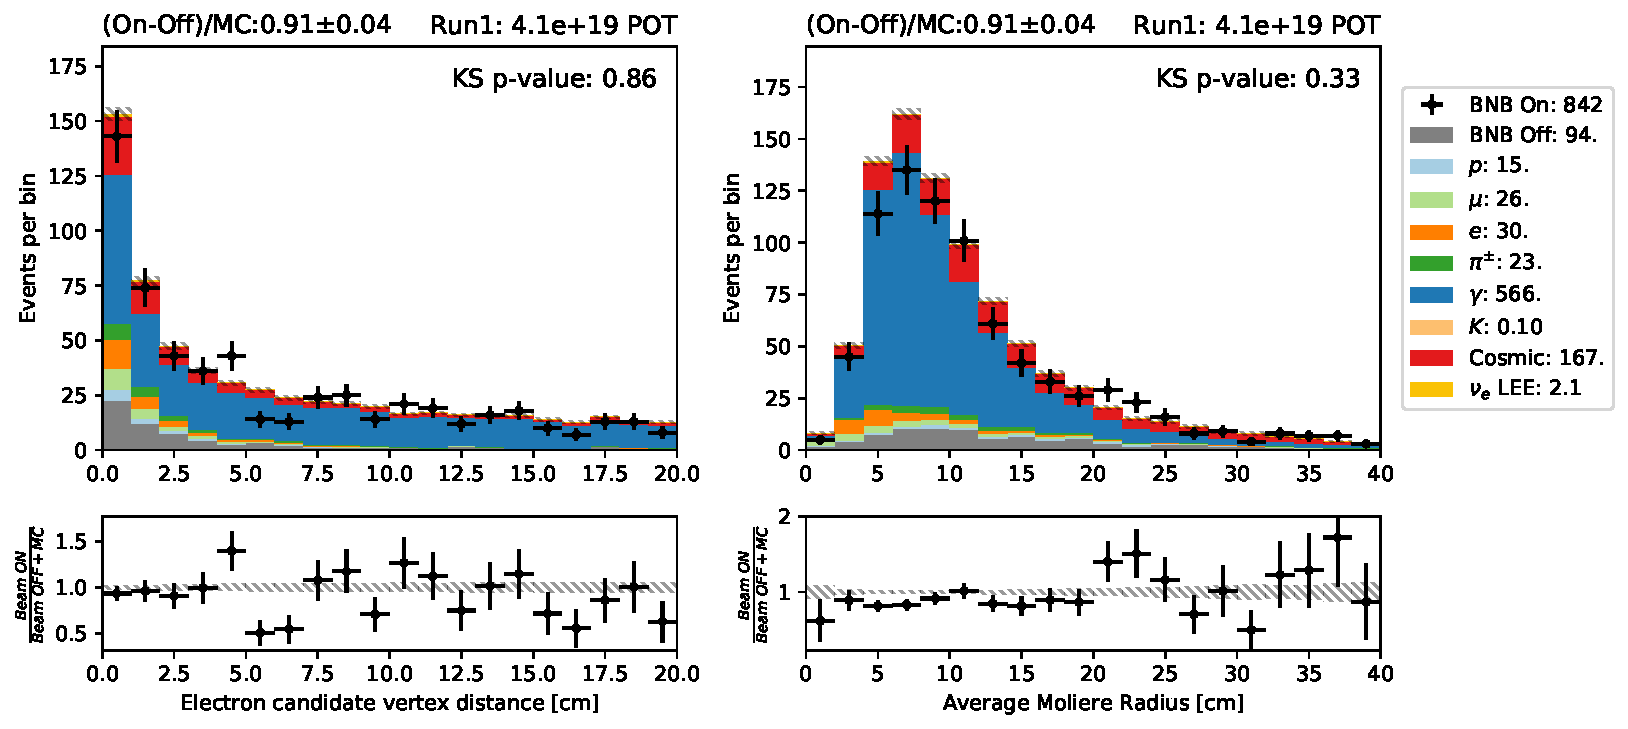
\includegraphics[width=\textwidth]{NueCCsel/Images/run1/e_cand_dist.pdf}
    \caption{Caption}
    \label{fig:e_cand_dist}
\end{figure}

\begin{figure}
    \centering
    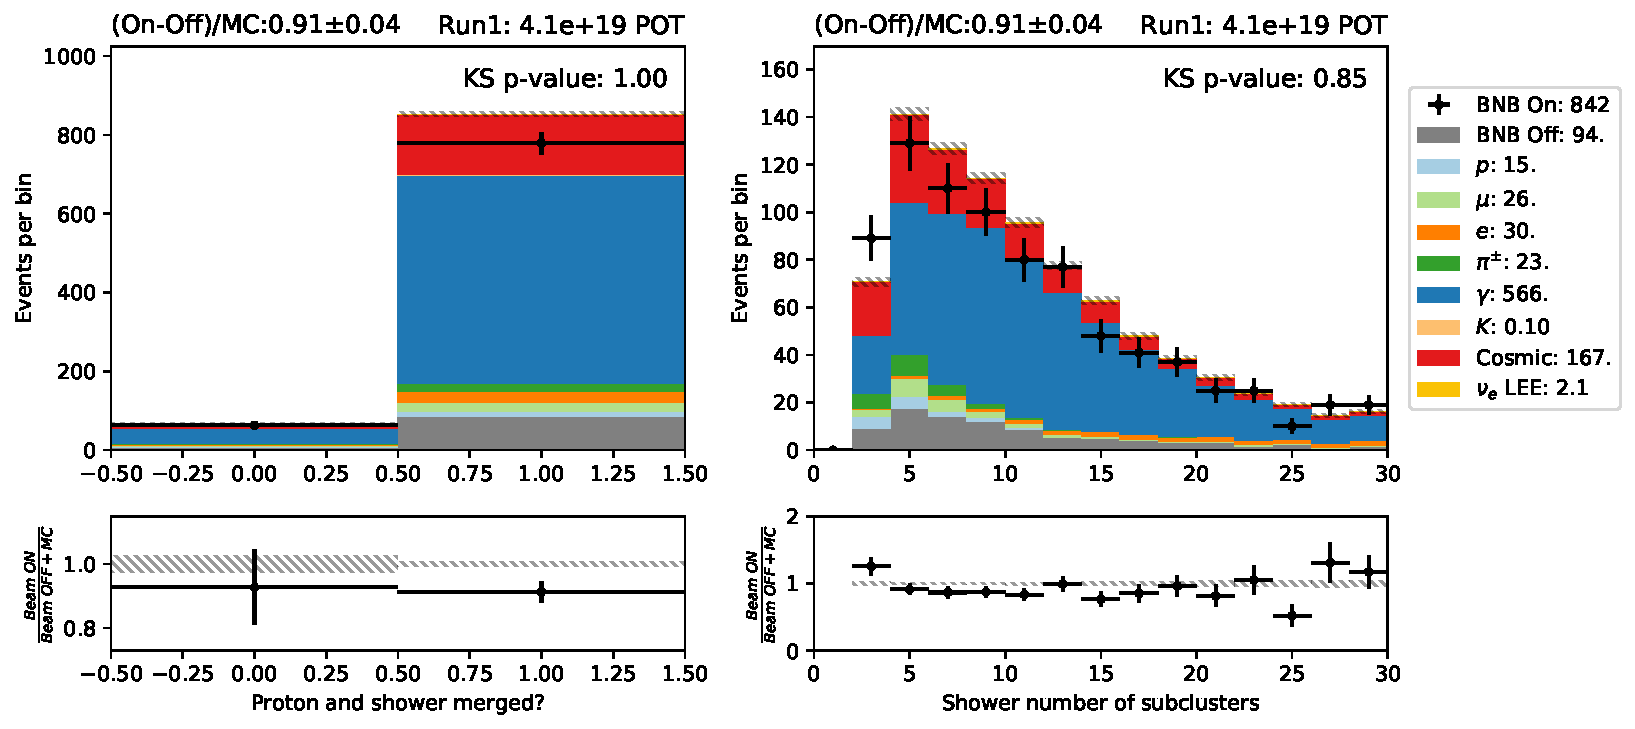
\includegraphics[width=\textwidth]{NueCCsel/Images/run1/e_cand_subclusters.pdf}
    \caption{Caption}
    \label{fig:e_cand_subclusters}
\end{figure}

\begin{figure}
    \centering
    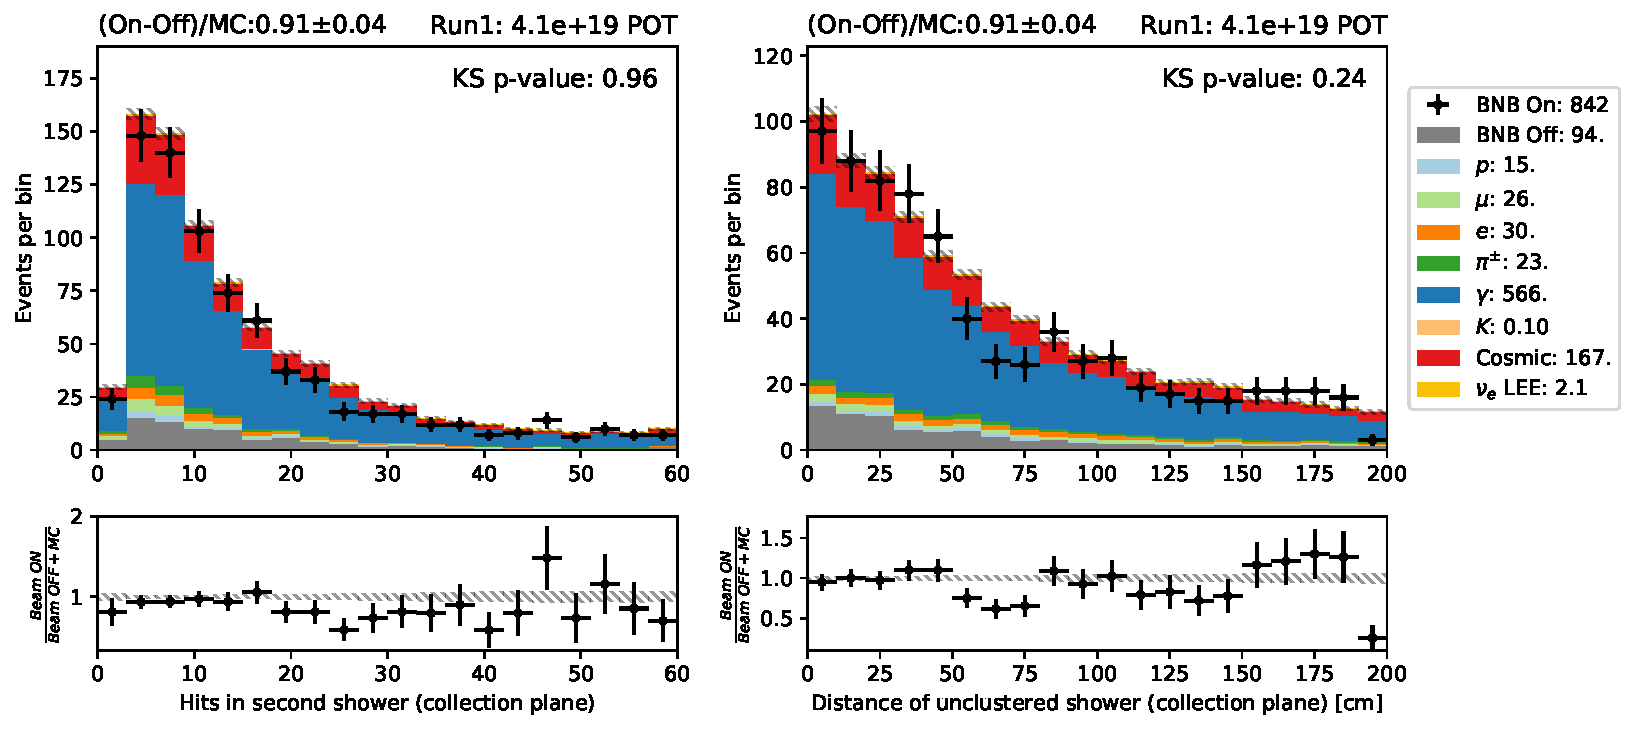
\includegraphics[width=\textwidth]{NueCCsel/Images/run1/e_cand_secondshower.pdf}
    \caption{Caption}
    \label{fig:e_cand_secondshower}
\end{figure}

\begin{figure}
    \centering
    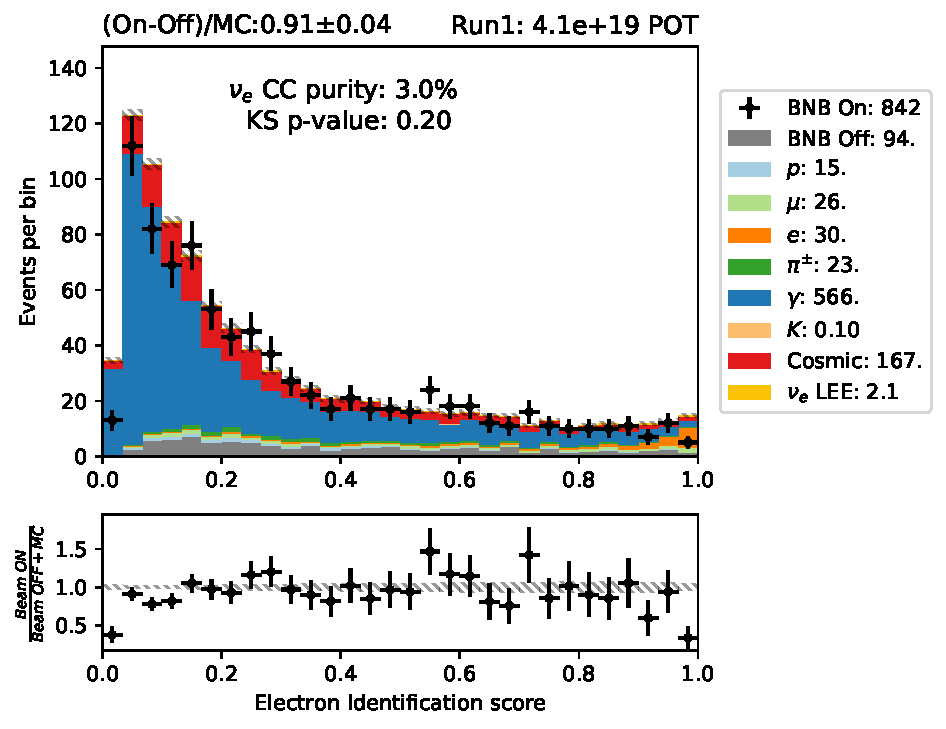
\includegraphics[width=0.5\textwidth]{NueCCsel/Images/run1/pre_e_score.pdf}
    \caption{Caption}
    \label{fig:pre_shower_E_pdg}
\end{figure}


\subsubsection{Other Daughters}

\begin{figure}
    \centering
    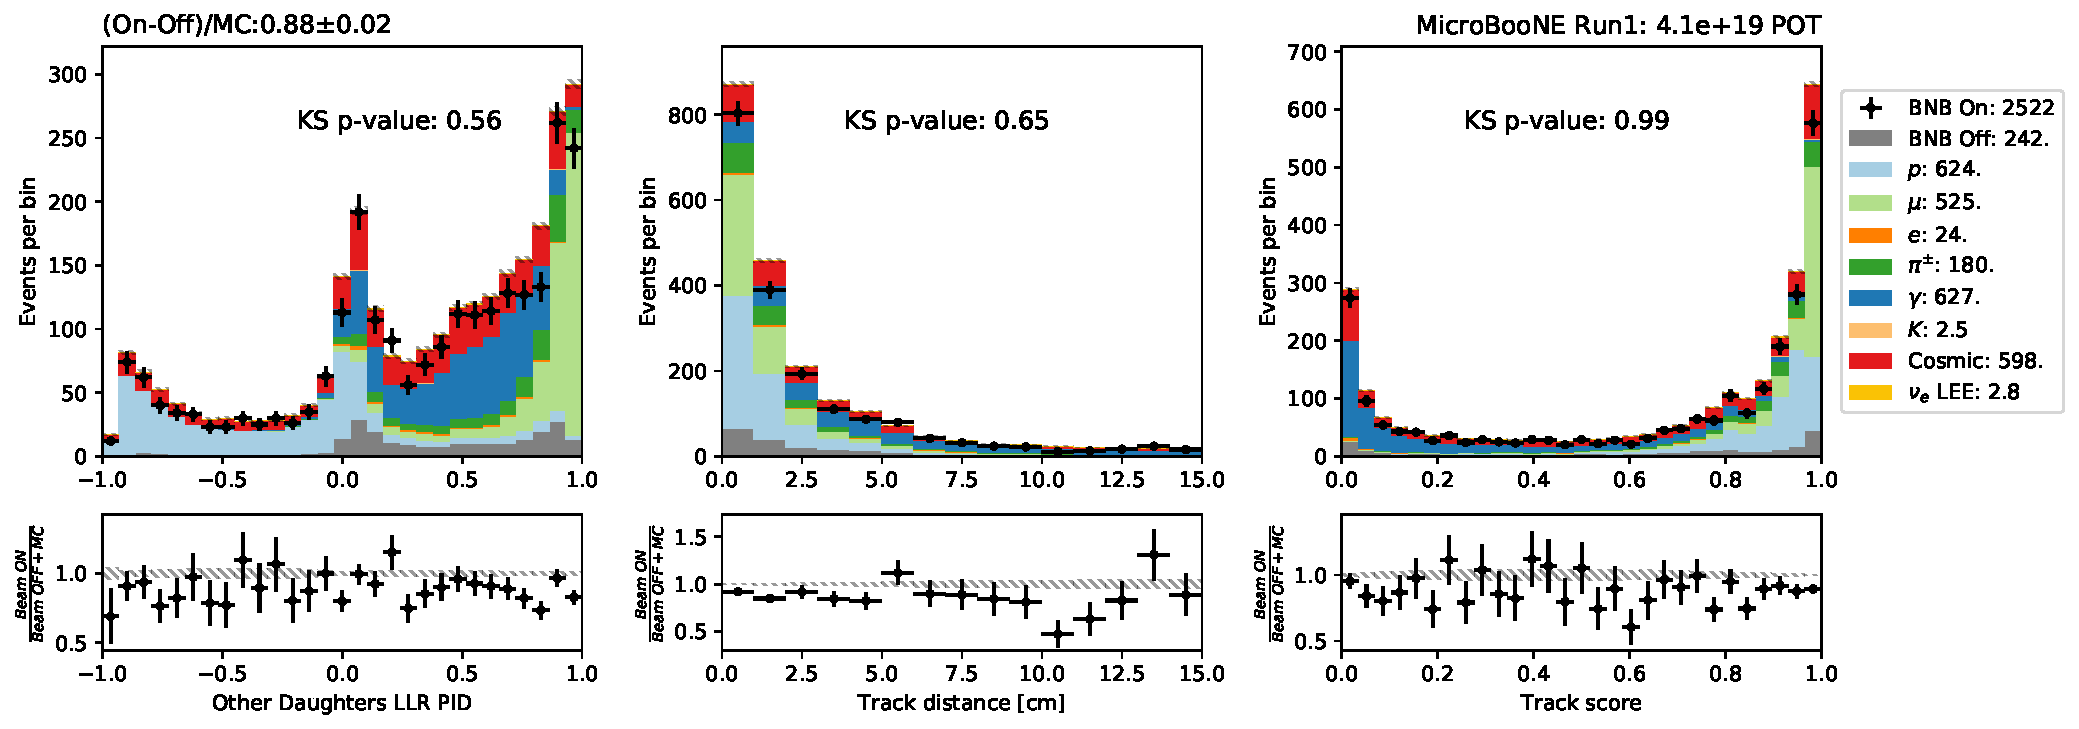
\includegraphics[width=\textwidth]{NueCCsel/Images/run1/pre_daughter_1.pdf}
    \caption{Caption}
    \label{fig:pre_daughter_1}
\end{figure}

\begin{figure}
    \centering
    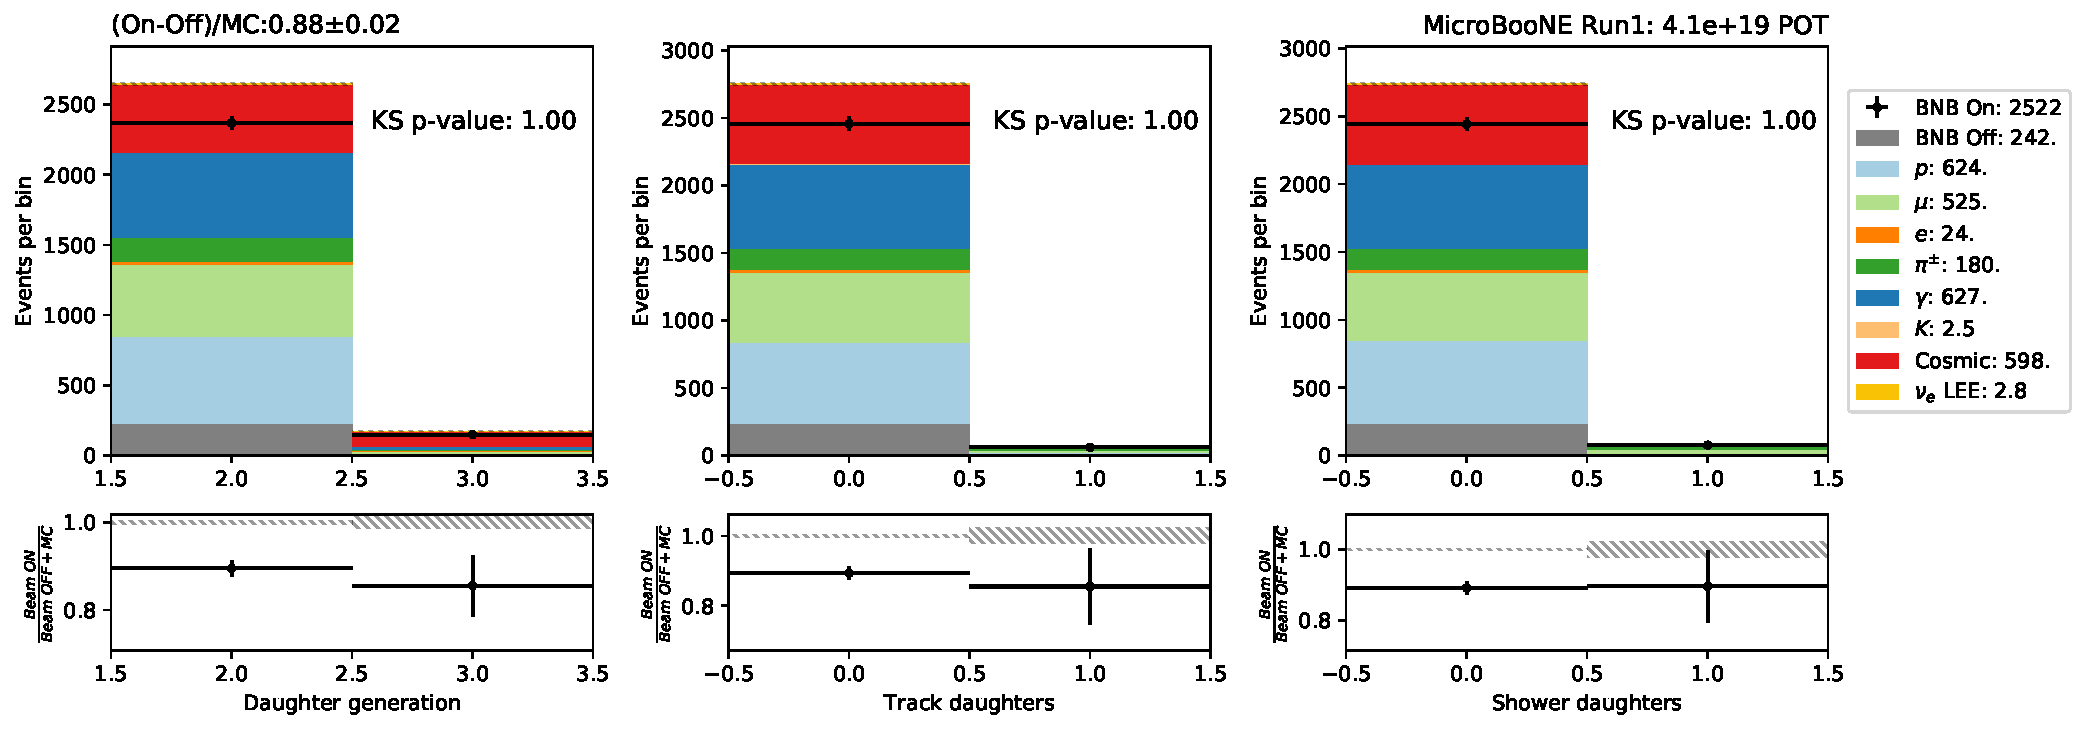
\includegraphics[width=\textwidth]{NueCCsel/Images/run1/pre_daughter_2.pdf}
    \caption{Caption}
    \label{fig:pre_daughter_2}
\end{figure}

\begin{figure}
    \centering
    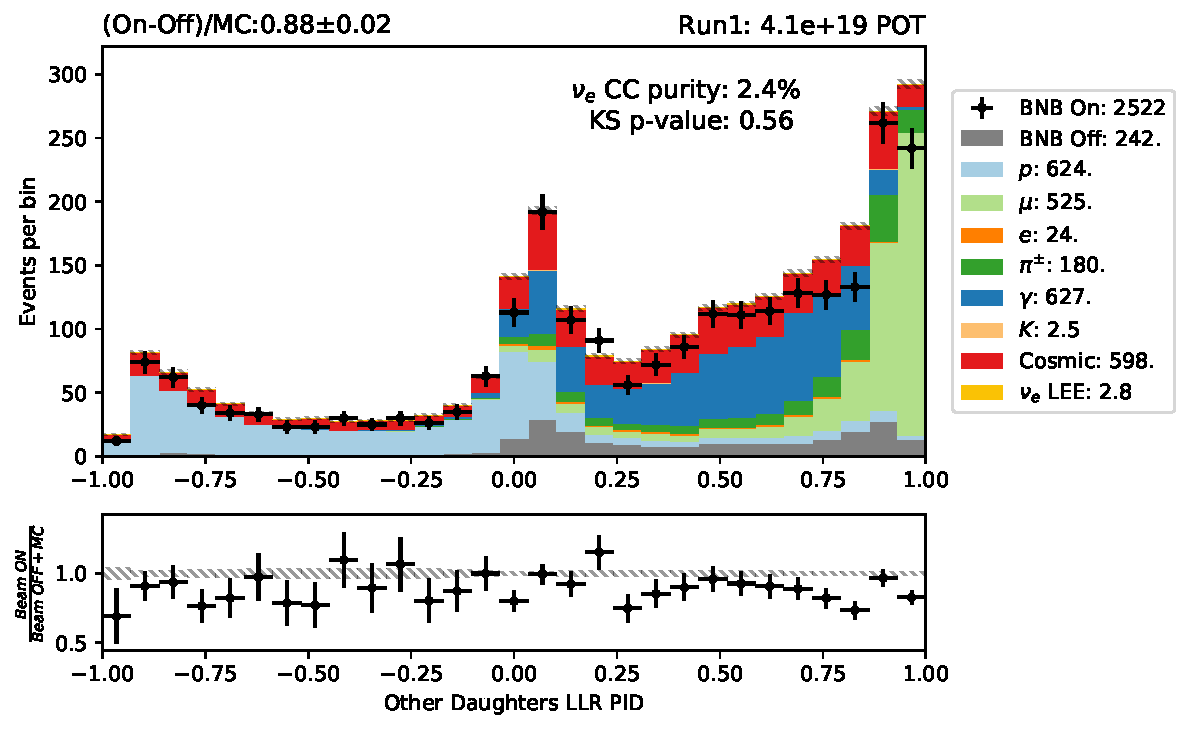
\includegraphics[width=0.5\textwidth]{NueCCsel/Images/run1/pre_daughter_pid.pdf}
    \caption{Caption}
    \label{fig:pre_daughter_pid}
\end{figure}

\begin{figure}
    \centering
    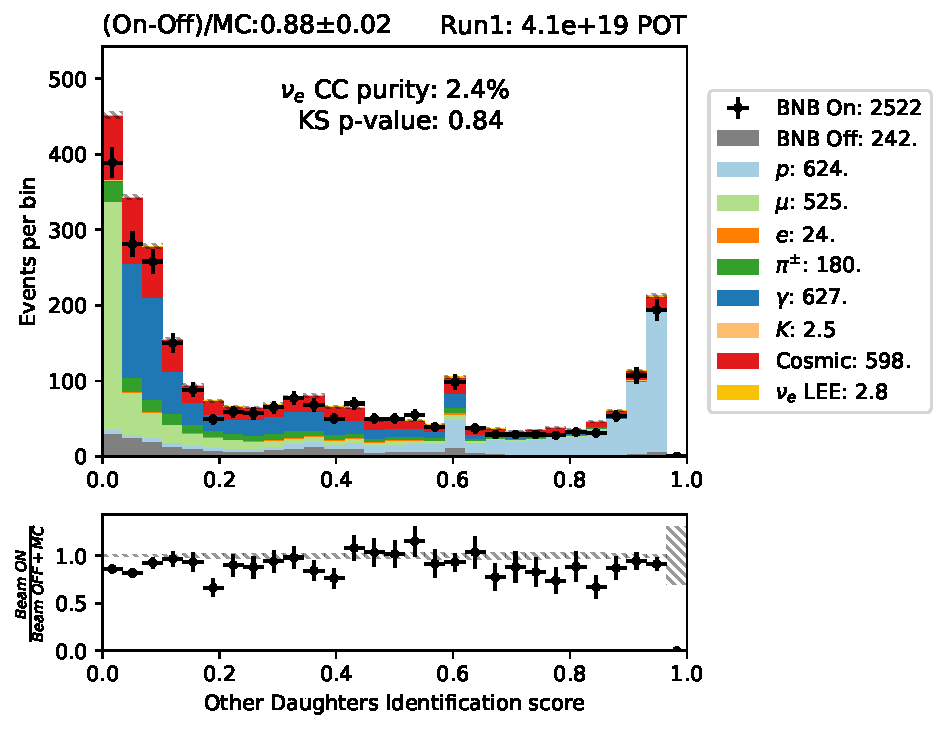
\includegraphics[width=0.5\textwidth]{NueCCsel/Images/run1/pre_daughter_score.pdf}
    \caption{Caption}
    \label{fig:pre_daughter_score}
\end{figure}

\subsubsection{Event Selection}

\begin{figure}
    \centering
    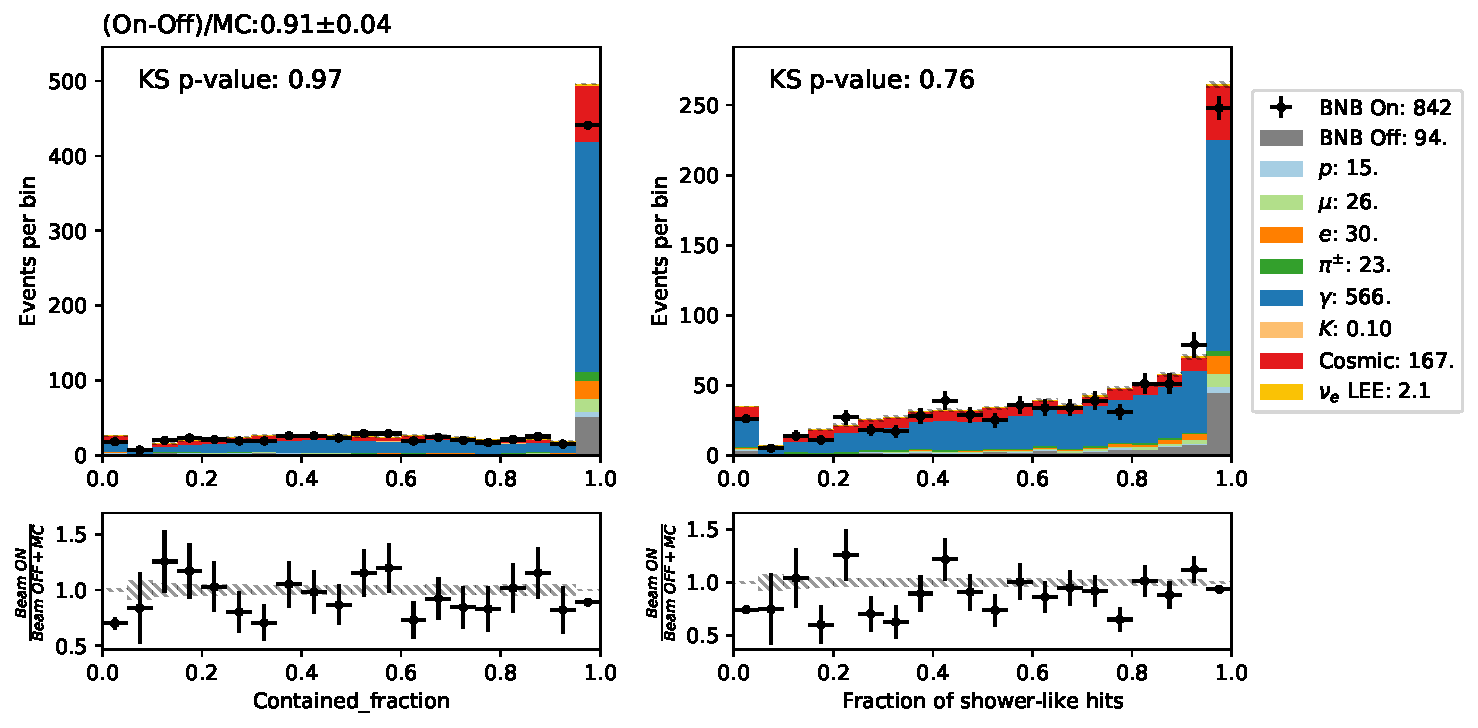
\includegraphics[width=\textwidth]{NueCCsel/Images/run1/bdt_1.pdf}
    \caption{Caption}
    \label{fig:bdt_1}
\end{figure}

\begin{figure}
    \centering
    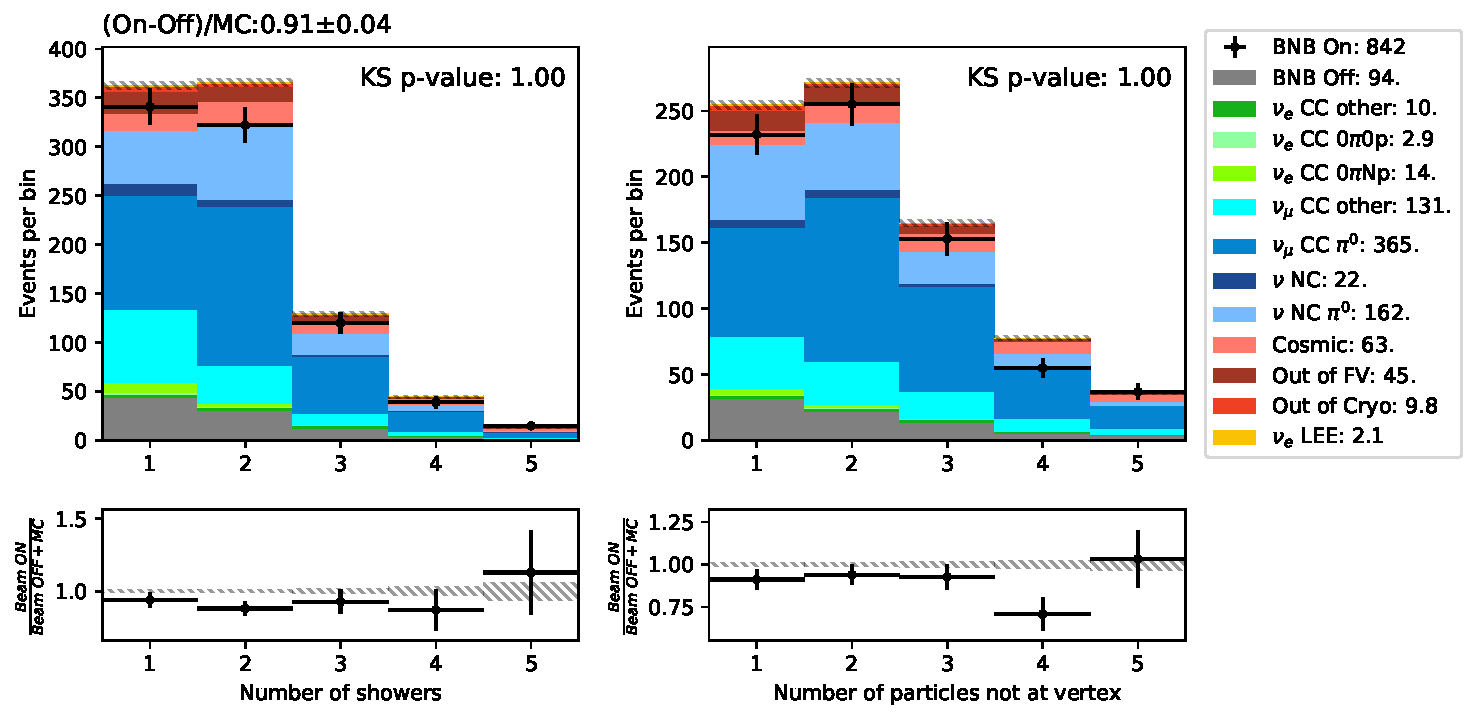
\includegraphics[width=\textwidth]{NueCCsel/Images/run1/bdt_2.pdf}
    \caption{Caption}
    \label{fig:bdt_2}
\end{figure}

\begin{figure}
    \centering
    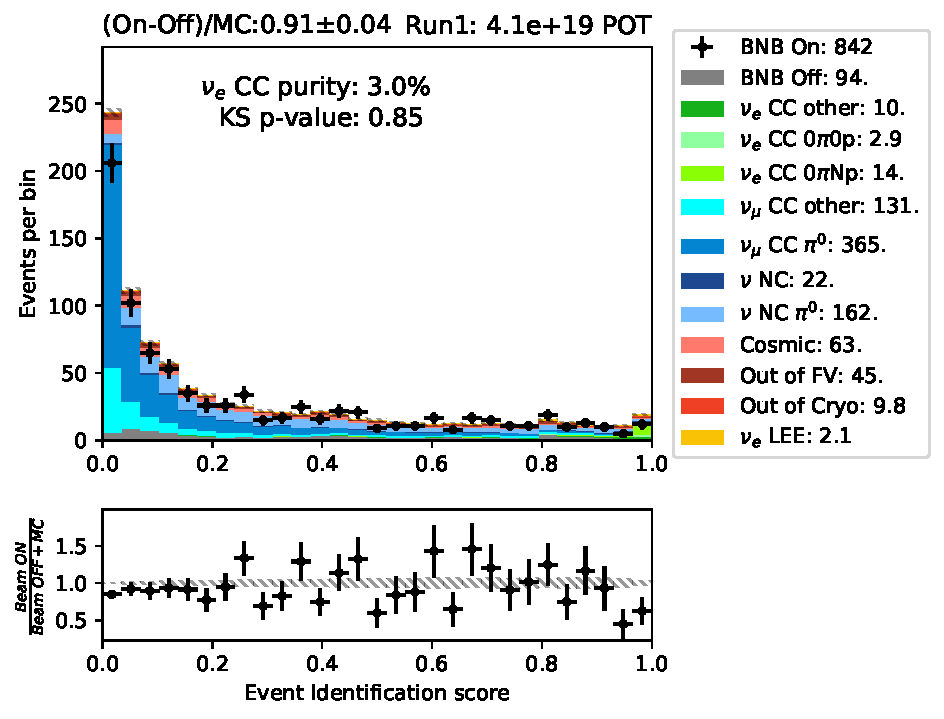
\includegraphics[width=0.495\textwidth]{NueCCsel/Images/run1/pre_event_score.pdf}
    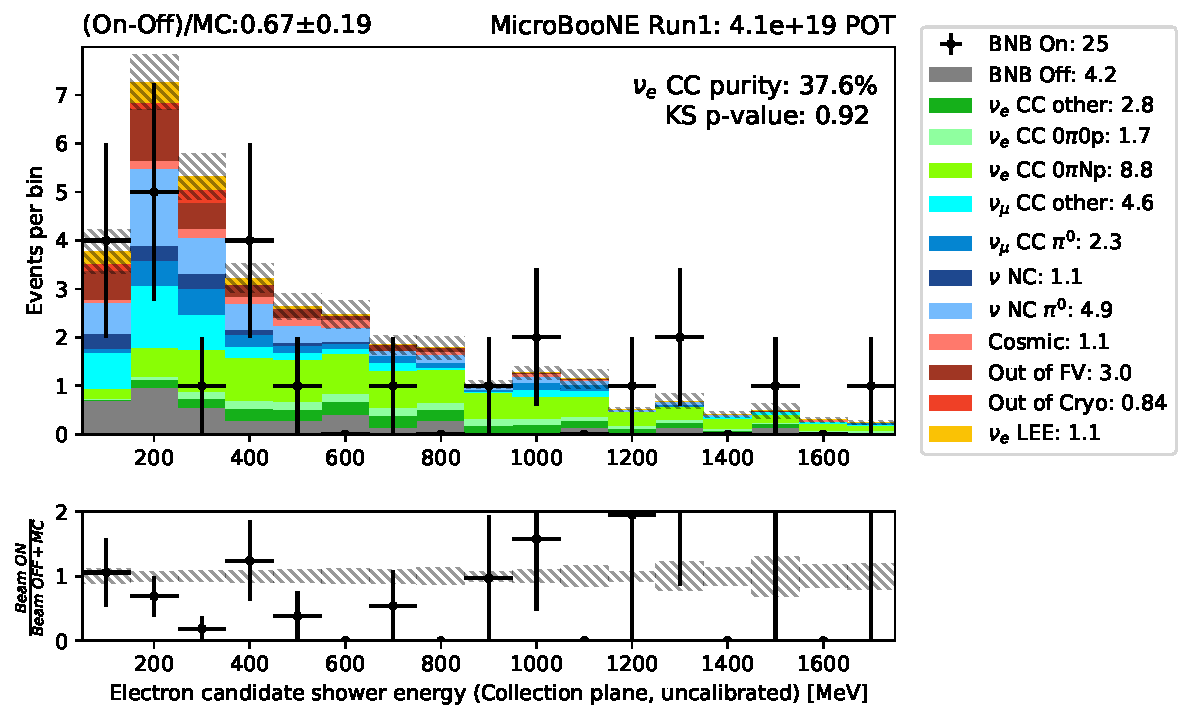
\includegraphics[width=0.495\textwidth]{NueCCsel/Images/run1/nue_shower_energy_y.pdf}
    \caption{Caption}
    \label{fig:pre_daughter_score}
\end{figure}


